\chapter{Android}
\label{android}

% http://www.tutorialspoint.com/android/
% http://www.android-app-market.com/android-architecture.html
% http://www.slideshare.net/trailukya_dutta/know-about-android-operating-system
% http://www.slideshare.net/rizzuIT/android-os-28305291
Neste capitulo é apresentado o sistema operacional Android, pois o mesmo é proposto 
como base para os dispositivos que executarão a localização baseada em RSS \textit{fingerprinting}.

O Android é um sistema operacional baseado no núcleo do Linux para dispositivos móveis, 
desenvolvido pela \textit{Open Handset Alliance}, liderada pela Google e composta por
outras empresas, tais como: Intel, Nvidia, Samsung, LG, entre outras \cite{android0}. 
O código fonte do sistema operacional está sobre a licença do Apache \cite{apacheLicence}. 

Ele apresenta vários recursos que podem facilmente empregados na robótica como
câmeras, GPS, aceleradores gráficos 2D e 3D, \textit{bluetooth}, wifi e também
suporta diversos sensores como barômetro, magnetômetro, acelerômetro, 
 sensor de proximidade, sensor de pressão, termômetro e compasso. 
 
 Este sistema operacional está presente em centenas 
de milhões de aparelhos em mais de 190 países \cite{androidDev} e possui um rico
ambiente de desenvolvimento provido pelo Android SDK \cite{sdk}, incluindo um emulador de dispositivo, 
ferramentes de depuração, memória, performance e um \textit{plugin} para o Eclipse (ADT). 
A seguir, são apresentadas a arquitetura desse sistema operacional 
e os componentes de uma aplicação Android.

\clearpage
\begin{comment}
- Application framework proporciona a reutilização e substituição de componentes
- Dalvik virtual machine optimizada para dispositivos móveis
- Browser Integrado baseado no Webkit engine
- Gráficos Optimizados possui uma biblioteca 2D; e 3D baseada na especificação OpenGL ES 1.0 (aceleração de hardware é opcional)
- SQLite para guardar dados estruturados
- Suporte multimídia para audio, video e formatos de imagem (MPEG4, H.264, MP3, AAC, AMR, JPG, PNG, GIF)
- Telefonia GSM (dependente de hardware)
- Bluetooth, EDGE, 3G, e WiFi (dependente de hardware)
- Camera, GPS, compasso, e acelerômetro (dependente de hardware)
- Rico ambiente de desenvolvimento Android SDK and NDK, 
incluindo um emulador de dispositivo, ferramentes de depuração,
memória, performance e um plugion para o Eclipse (ADT)
 - cameras, touchscreen, GPS, acelerômetro, giroscópio, barômetro, magnetômetro,
 sensor de proximidade, sensor de pressão, termometro, aceleradores graficos 2D e 3D.
 
\end{comment}
\section{Arquitetura}
  A arquitetura do Android é composta por cinco camadas, sendo elas: aplicações, 
  \textit{framework} de aplicações (\textit{applications}), \textit{android runtime}, bibliotecas (\textit{libraries}) e kernel Linux.
  A figura abaixo mostra a disposição dessas camadas:
\begin{figure}[hb]
\centering
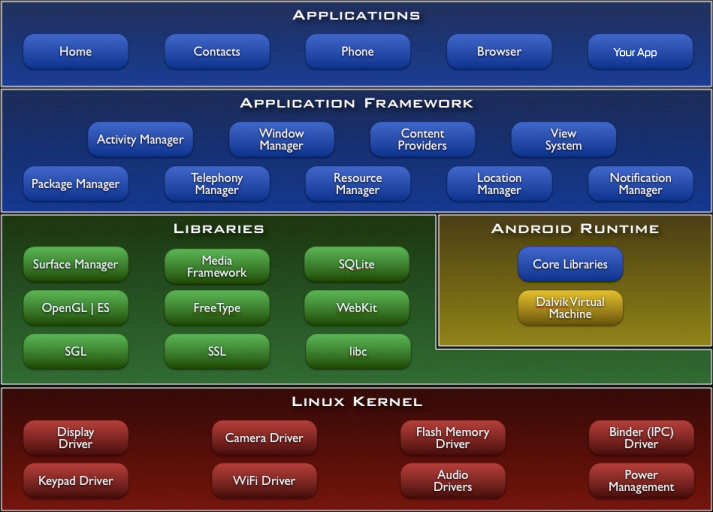
\includegraphics[scale=0.45]{images/Android-architecture.jpg}
\caption{Arquitetura Android\cite{android1}. }
\label{fig:android-arc}
\end{figure}
	
	
\subsection{Aplicações}
 A camada de aplicações comporta todos aplicativos instalados no sistema operacional, a maioria delas escritas em java.
Junto com o Android vai um conjunto de aplicações fundamentais. São elas: cliente de email, clente de SMS, agenda, gerenciador de contatos (Contacts),
mapas e navegador (Browser).
% (as long as the users of your app permits it). 

\subsection{\textit{Framework} de Aplicações}
  Esta camada fornece vários componentes essenciais do sistema para as aplicações em forma de classes Java \cite{android1}. 
  Eles gerenciam funções básicas do aparelho, os principais componentes disponíveis são:
  \begin{itemize}
   \item \textit{Activity Manager}: gerencia o ciclo de vida de uma \textit{activity} \cite{activity}, explicado em 
   mais detalhes na seção 4.2.1.
   \item \textit{Content Providers}: faz o compartilhamento de dados entre aplicações.
   \item \textit{Telephony Manager}: gerencia todas as ligações telefônicas.
   \item \textit{Location Manager}: controla os sistemas de localização como GPS e torre celular.
   \item \textit{Resource Manager}: fornece alguns recursos utilizadas por uma aplicação como \textit{strings}, imagens, arquivos de \textit{layout}, 
   arquivos de áudio e vídeo.
  \end{itemize}

   A arquitetura de aplicações foi projetada para simplificar o reuso de componentes, qualquer aplicação publica suas funcionalidades e uma
    outra aplicação pode fazer uso delas (sujeito as regras de segurança impostas pelo \textit{framework}) \cite{android0}. Essa estrutura permite que os componentes 
    sejam substituídos pelo usuário.
    
\subsection{Bibliotecas}

O Android inclui um conjunto de bibliotecas nativas utilizadas por vários componentes do sistema. 
Elas foram implementada em C/C++, mas são acessadas através de interfaces Java \cite{android0} 
disponibilizada pelo \textit{Framework} de aplicações.
 Abaixo, algumas das principais bibliotecas:
  \begin{itemize}
   \item \textit{System C library}: uma implementação derivada da biblioteca C padrão sistema (libc) do BSD otimizada para dispositivos móveis.
   \item \textit{Media Libraries}: baseado no PacketVideo’s OpenCORE; as bibliotecas suportam os mais populares formatos de audio e video, bem como imagens estáticas.
   \item \textit{Surface Manager}: gerencia o acesso a tela do aparelho bem como as múltiplas camadas de aplicações 2D e 3D.
   \item \textit{LibWebCore}:  \textit {web browser engine} utilizado no Chrome(navegador padrão do Android).
   \item \textit{3D libraries}: uma implementação baseada no OpenGL ES 1.0 \cite{openGL}; as bibliotecas utilizam aceleração 3D via \textit{hardware}; 
   ou o \textit{software} de renderização 3D altamente otimizado incluído no Android.
   \item SGL – o motor gráfico 2D.
   \item \textit{FreeType}: faz renderização de fontes bitmap e vector.
   \item SQLite – um poderoso e leve \textit{engine} de banco de dados.
  \end{itemize}

\begin{comment}
Surface Manager: It is used for compositing window manager with off-screen buffering.
Off-screen buffering means you cant directly draw into the screen, but your drawings go to the off-screen buffer. 
There it is combined with other drawings and form the final screen the user will see. 
This off screen buffer is the reason behind the transparency of windows.
\end{comment}

\subsection{\textit{Android Runtime}}

O Android inclui um grupo de bibliotecas que fornece a maioria das 
funcionalidades disponíveis nas principais bibliotecas da linguagem Java.
Esta camada possui um componente chave do Android chamada máquina virtual Dalvik, 
ela é uma maquina virtual java  baseada em registros especificamente projetada pra o Android \cite{android1} e otimizada
 para aparelhos que utilizam bateria e possuem memória e CPU limitados.
Toda aplicação Android roda em seu próprio processo, com sua própria instância da máquina virtual Dalvik.

Apesar de que a maioria das aplicações Android serem escritas em Java, 
Java \textit{byte code} não é suportado pela Dalvik.
As classes Java são compiladas em arquivos .dex(``Dalvik \textit{executable}''), 
que são otimizados para consumo mínimo de memória,
através da ferramenta ``dx'' incluída no SDK \cite{android0}.

A Dalvik foi desenvolvido de forma a executar várias maquinas virtuais simultâneas eficientemente, 
fornecendo segurança e isolamento. O gerenciamento de memória
e o suporte a \textit{multi-threading} são feitos pelo kernel Linux. 

A segurança entre aplicações e o sistema, é forçada pelos níveis de execução de 
processos do Linux\cite{niveisExec} e cada aplicações ganha um id de usuário e grupo, um 
aplicativo só pode acessar um arquivo no qual pertença a seu usuário. 
Os aplicativos só podem acessar recursos do sistema nos quais forem previamente 
permitidos pelo usuário do aparelho na instalação do aplicativo.

  Apesar de utilizar o Linux como base, a portabilidade de aplicativos Linux
   para Android não é simples, pois ele não possui o sistema de janelas X, 
   nem suporte completo ao conjunto padrão de bibliotecas GNU.
\begin{comment}
It is a type of JVM used in android devices to run apps and is optimized for low processing power and low memory environments. 
Unlike the JVM, the Dalvik Virtual Machine doesn’t run .class files, instead it runs .dex files. 
.dex files are built from .class file at the time of compilation and provides hifger efficiency in low resource environments. 
The Dalvik VM allows multiple instance of Virtual machine to be created simultaneously providing security, isolation, memory management and threading support. 
It is developed by Dan Bornstein of Google.


Core Java Libraries
These are different from Java SE and Java ME libraries. However these libraries provides most of the functionalities defined in the Java SE libraries.
\end{comment}

\subsection{Linux Kernel}

A camada base da arquitetura do Android é o kernel Linux com algumas alterações feitas pela Google. 
As versões correntes do sistema operacional utilizam o kernel Linux 3.x como base, enquanto que os dispositivos 
 com a versão do sistema operacional inferior a o 4.0 (\textit{Ice Cream Sandwich}) são baseados no kernel Linux 2.6.x \cite{android1}.

O kernel Linux é responsável por executar os serviços centrais do sistema, onde o Linux é realmente bom, como segurança, gerenciamento de processos, 
memória e rede. Ele também fornece suporte a uma vasta quantidade \textit{drivers} essenciais para \textit{hardwares} periféricos como câmera, teclado, 
tela, \textit{bluetooth}, facilitando a portabilidade do Android para diferentes tipos de \textit{hardwares}. 
Assim, essa camada faz a interface com o hardware do aparelho.

\begin{comment}
At the bottom of the layers is Linux - Linux 2.6 with approximately 115 patches. 
This provides basic system functionality like process management, memory management, device management like camera, keypad, display etc. 
Also, the kernel handles all the things that Linux is really good at such as networking and a vast array of device drivers, 
which take the pain out of interfacing to peripheral hardware.
Utiliza a versão 2,6 do kernel do Linux para os serviços centrais do sistema, tais como segurança, gestão de memória, gestão de processos, etc. 
O kernel também atua como uma camada de abstração entre o hardware e o resto do software.
As of November 2013, current Android versions consist of a kernel based on the Linux kernel version 3.x, 
while Android versions older than 4.0 Ice Cream Sandwich were based on the Linux kernel 2.6.x.

The basic layer is the Linux kernel. The whole Android OS is built on top of the Linux 2.6 Kernel with some further architectural changes made by Google. 
It is this Linux that interacts with the hardware and contains all the essential hardware drivers. 
Drivers are programs that control and communicate with the hardware. For example, consider the Bluetooth function. 
All devices has a Bluetooth hardware in it. Therefore the kernel must include a Bluetooth driver to communicate with the Bluetooth hardware.  
The Linux kernel also  acts as an abstraction layer between the hardware and other software layers. 
Android uses the Linux for all its core functionality such as Memory management, process management, networking, security settings etc. 
As the Android is built on a most popular and proven foundation, it made the porting of Android to variety of hardware, a relatively painless task.
\end{comment}
\section{Componentes de uma Aplicação}
  O código java compilado junto com outros recursos requeridos pela aplicação, são empacotados em um único arquivo com 
  extensão .apk (\textit{``Android Package''}), ele é quem será instalado no aparelho. 
  Tudo que esta contido neste arquivo é considerado uma aplicação Android \cite{android0}. 

  Um característica interessante do Android é que uma aplicação pode utilizar
  componentes de outra aplicação (desde que esta aplicação permita), sem que seja necessário incorporar
  o código ou criar um \textit{link} para este componente, basta inicializa-lo quando necessário. 

  Para que isso funcione, o sistema deve ser capaz de inciar um processo quando 
  esse componente é requirido, e também instanciar todos os objetos java desse componente.
  Ao contrario de aplicações de outros sistemas, as aplicações Android não possui um único 
  ponto de inicialização (não há função main(), por exemplo). Elas possuem componentes essenciais 
  que podem ser inicializados e executados sempre que forem necessários. Há quatro tipos desses componentes:
  \textit{activity}, \textit{service}, \textit{broadcast receiver} e \textit{content provider}, explicados 
  a seguir.
  
  Quando um componente precisa ser executado, o Android inicia um processo Linux com uma 
  única \textit{thread} (\textit{thread} principal). 
  Por padrão, todos os componentes de uma aplicação executam nesse processo 
  e nessa \textit{thread}, mas se necessário, 
  o sistema permite que componentes executem em outros processos, 
  e novas \textit{threads} possam ser instanciadas por qualquer processo. 
  
  As chamadas ao sistema são feitas pela \textit{thread} principal. 
  Como todos os componentes executam nessa \textit{thread}, 
  eles não devem realizar operações que levem muito tempo 
  para serem finalizadas (como a computação de laços ou operações envolvendo 
  internet), pois isso pode bloquear a execução de outros componentes do processo. 
  Operações que demandam de muito tempo devem ser 
  executadas em uma nova \textit{thread}.
  
  Cada componente tem suas características e comportamentos distintos, a seguir serão vistos em mais
  detalhes cada tipo de componente.
\begin{comment}
The process where a component runs is controlled by the manifest file. 
The component elements — <activity>, <service>, <receiver>, and <provider> 
— each have a process attribute that can specify a process where that component should run. 
These attributes can be set so that each component runs in its own process, or so that some components share a process while others do not. 
They can also be set so that components of different applications run in the same process — 
provided that the applications share the same Linux user ID and are signed by the same authorities.
The <application> element also has a process attribute, for setting a default value that applies to all components.

All components are instantiated in the main thread of the specified process, 
and system calls to the component are dispatched from that thread. Separate threads are not created for each instance.
This means that no component should perform long or blocking operations (such as networking operations or computation loops) 
when called by the system, since this will block any other components also in the process. 
You can spawn separate threads for long operations

 Android may decide to shut down a process at some point, when memory is 
 low and required by other processes that are more immediately serving the user. 
 Application components running in the process are consequently destroyed. 
 A process is restarted for those components when there's again work for them to do.

When deciding which processes to terminate, Android weighs their relative importance to the user. 
For example, it more readily shuts down a process with activities that are 
no longer visible on screen than a process with visible activities. 
The decision whether to terminate a process, therefore, 
depends on the state of the components running in that process. 
Those states are the subject of a later section
\end{comment}

\subsection{Activity}
 Uma \textit{activity} é um componente da aplicação que fornece uma tela na qual o usuário possa interagir \cite{activity}.
 Para cada \textit{activity} é dada uma janela na qual ela possa exibir seu elementos, uma janela pode ou não preencher toda a tela. 
 
 Uma aplicação frequentemente possui varias \textit{activities} que são ligadas umas ás outras.  
 Tipicamente, uma \textit{activity} é especificada como principal, ou seja, ela que exibida quando o usuário executa 
 a aplicação pela primeira vez. Cada \textit{activity} pode iniciar outra \textit{activities} pra realizar uma outra tarefa. 
 Toda vez que uma nova \textit{activity} é iniciada e apresentada(\textit{foreground}) ao usuário, a \textit{activity} anterior é ``parada'' e o sistema insere ela em uma pilha. 
 Quando o usuário pressiona o botão voltar, uma \textit{activity} é desempilhada e devolvida para a tela do usuário, e \textit{activity} anterior é destruída.
 
 O componente \textit{activity} possui um ciclo de vida especial, definido por um conjunto de estados implementado por 
 um sistema em cascata de chamada de métodos específicos. Abaixo o esquema de transição desses estados:
 \clearpage
 \begin{figure}[hb]
\centering
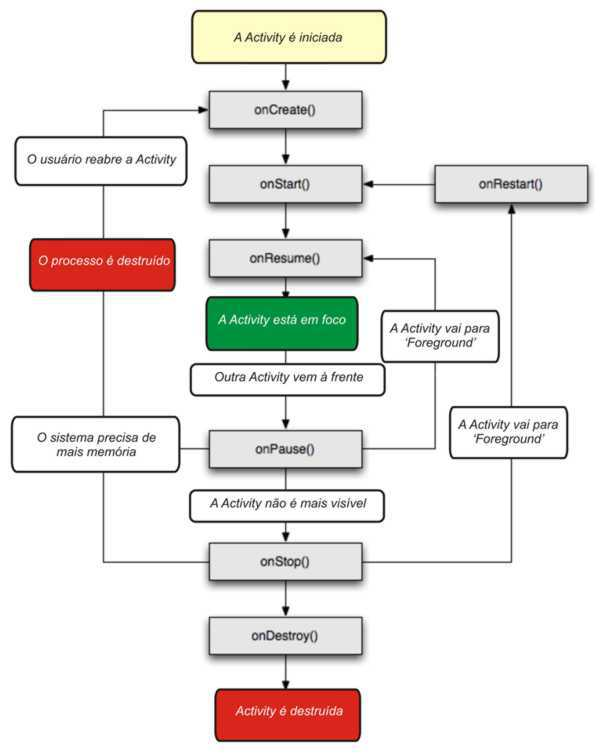
\includegraphics[scale=0.6]{images/activity-ciclo-de-vida.jpg}
\caption{Ciclo de vida de uma \textit{activity}\cite{android1}. }
\label{fig:activity-lifecycle}
\end{figure}

Os métodos que representam os estado do ciclo de vida tem as seguintes funções:
\begin{itemize}
 \item \textbf{onCreate():} é chamado uma única vez, este método 
 é responsável por construir a tela que será apresentada.
 \item \textbf{onStart():} é chamado quando a \textit{activity} está prestes a ficar visível para o usuário.
 \item \textbf{onResume():} é chamado quando a \textit{activity} é visível para o usuário.
 \item \textbf{onRestart():} este método é chamado quando a \textit{activity} foi temporariamente parada e está 
 sendo reiniciada.
 \item \textbf{onPause():} é chamado quando a \textit{activity} esta sendo encerrada, e não está mais visível ao usuário.
 \item \textbf{onStop():} é chamado quando a \textit{activity} está sendo encerrada.
 \item \textbf{onDestroy():} este encerra a execução de uma \textit{activity}.
\end{itemize}
 
\subsection{Services}
Um \textit{service} não possui interface visual, pois sua função é 
executar tarefas em segundo plano por um período de tempo indefinido \cite{service}, 
mesmo que o usuário troque de aplicação o \textit{service} continua sua execução.
Por exemplo, um \textit{service} pode tocar uma musica em segundo plano, buscar alguma informação na rede 
ou calcular algo e entregar o resultado para uma \textit{activity} que precise. 

  Os \textit{services} disponibilizam uma interface que permite que mesmo em execução outros componentes possam se comunicar com ele, 
  isso possibilita fazer comunicações entre processos \cite{service}.
  Por exemplo, para um \textit{service} responsável por tocar uma lista de musicas, isso seria útil, pois permitiria que o usuário pausasse, parasse e 
  recomeçasse a execução da lista.
  
  Como os outros componentes \textit{services} executam na \textit{thread} principal. Então para não bloquear outros componentes 
  ou a interface do usuário, frequentemente eles inciam outra \textit{thread} para realizar tarefas que levam muito tempo para serem concluídas. 
\subsection{Broadcast Receiver}
\textit{Broadcast receiver} é um componente que recebe e responde a notificações \cite{receiver}. %certos eventos
Muitas dessas notificações são emitidas pelo sistema operacional como mudança de fuso horário, 
carga da bateria está baixa, uma foto foi retirada ou o usuário mudou a linguagem corrente.
Qualquer aplicações pode também emitir notificações.

Uma aplicações pode ter diversos \textit{broadcast receivers} 
e responder a várias notificações que ela considere importante. Todos os \textit{receivers} 
herdam da classe BroadcastReceiver. Tipicamente eles não fazem nenhum processamento sobre a 
informação recebida, um \textit{broadcast receivers} deve iniciar uma \textit{activity} ou um \textit{service} para 
responder a notificação recebida.

\subsection{Content Providers}
Um \textit{content provider} faz com que um conjunto de dados da aplicação fique disponível para outra aplicações \cite{provider}. 
Eles são a única maneira de compartilhar dados entre aplicações. Ou seja, para tornar os dados públicos, só há duas maneiras: 
criando um \textit{content provider}
(uma subclasse ContentProvider) ou adicionando os dados em provedor existente -
se existe um que controle o mesmo tipo de dados e se tenha permissão para escrever nele.

O \textit{content provider} criado a partir da classe ContentProvider, implementa um conjunto de métodos
 que possibilita outras aplicações acessar e salvar dados do tipo que ele controla. No entanto, as aplicações 
 não acessam esses métodos diretamente. Para isso, elas devem utilizar um objeto da classe ContentResolver. 
 Onde este pode se comunicar com qualquer \textit{content provider}, eles cooperam para gerenciar a comunicação 
 entre processos envolvidos.
 
O Android fornece um conjunto de \textit{content providers} para dados comuns como 
áudio, vídeo, imagens e informações dos contatos. As aplicações podem acessar esses \textit{providers} 
para obter os dados que eles contem, para alguns é necessário obter permissões especias para ler os dados.

Os dados podem ser armazenados no sistema de arquivos ou em um banco de dados SQLite. 
\textit{Content providers} apresentam seus dados como uma tabela de um banco de dados, 
onde cada linha é um registro e cada coluna é um dado de um tipo particular. 


Em resumo este capitulo apresentou as principais características do sistema operacional base para o desenvolvimento do 
sistema de localização proposto no presente trabalho.